\section{Case Study 2}

The second case study implements the same system prototype for a movie ticket reservation system as seen in the pilot study. However, a different set of microservice design patterns is explored this time, including a significant change in inter-service communication style from synchronous REST request/response to asynchronous messaging.

\subsection{Design and Implementation}

\begin{figure}[H]
  \centering
  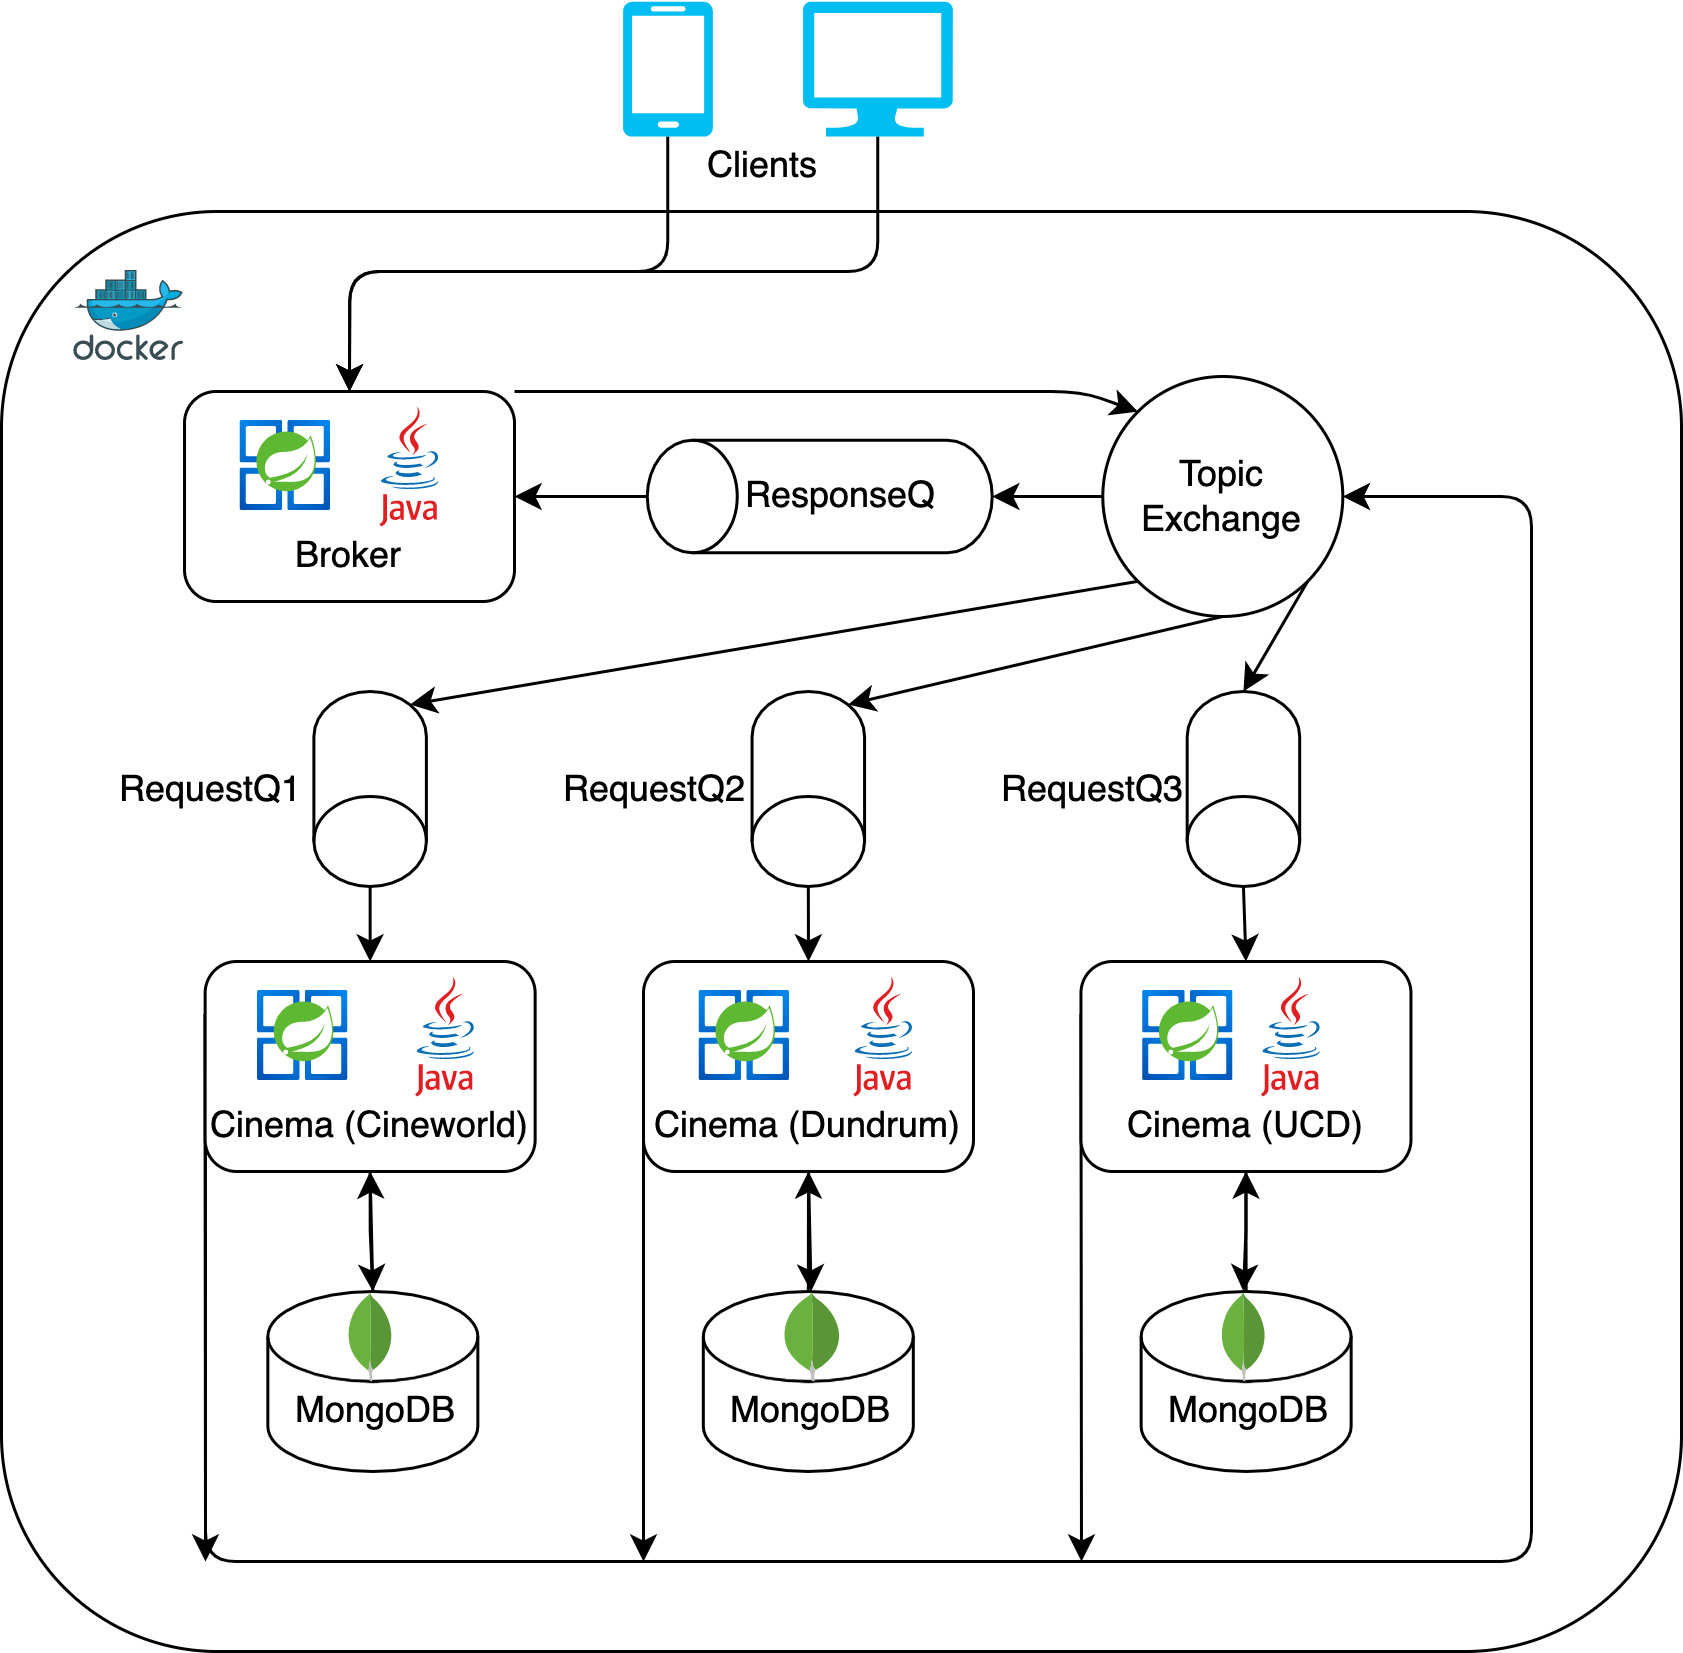
\includegraphics[width=0.6\linewidth]{./assets/diagrams/cs02-arch.png}
  \caption{System design for the second case study.}
  \label{fig:cs02-arch}
\end{figure}

The system architecture shown in Fig. \ref{fig:cs02-arch} is similar to the previous study's architecture in the sense that the three cinemas are still independent microservices with separate MongoDB database connections. However, the intermediary that intercepts client requests has been changed from an API gateway plus aggregator setup, to a message broker, that uses message queues to communicate with other services. For external clients, the broker still exposes a modified REST API, but with separate endpoints to send a request and fetch a response. Requests are hence made asynchronous from the client's perspective too, since a single endpoint is no longer expected to deliver results while maintaining an open connection. The design patterns implemented by this web application are described in detail here:


\subsubsection{Asynchronous Messaging}

For inter-service communication, the \textit{asynchronous messaging} is the recommended design pattern over synchronous request/response. Although external clients should still avail of a synchronous REST API to contact the intermediary (broker), the internal cinema services should communicate with the broker asynchronously to prevent blocking. There exist multiple realisations of this pattern, including the use of notifications, HTTP polling, publish/subscribe, or messaging queues request/response.

In this case study, RabbitMQ \footnote{\url{https://www.rabbitmq.com}}, a widely popular open-source asynchronous messaging technology, is the tool of choice. RabbitMQ implements AMQP (Advanced Message Queueing Protocol), a wire-level message-oriented middleware protocol with defining features such as message orientation, queueing, routing (point-to-point and publish/subscribe), reliability and security. The Spring AMQP \footnote{\url{https://spring.io/projects/spring-amqp\#overview}} project is used to greatly reduce the amount of boilerplate code required for infrastructure setup, by providing high-level abstractions: a Listener container asynchronously processed inbound messages, RabbitTemplate is used to send/receive messages, RabbitAdmin auto-declares queues, exchanges and bindings.

The main components of the messaging infrastructure are:
\begin{itemize}
  \item \textit{Request queues} - Every cinema microservice is configured to receive requests from the broker via a corresponding request queue.
  \item \textit{Response queue} - All cinema services send responses to a common response queue, that the broker consumes from before returning responses to the client.
  \item \textit{Topic exchange} - An exchange in RabbitMQ is a routing agent, for directing messages to/from different queues using header attributes, bindings and routing keys. A single topic exchange (given name: \code{cinema}) is used in this application, that is appropriate for messaging based on pre-defined "patterns" of routing keys as described below.
  \item \textit{Bindings and routing keys} - Bindings are used to link the four queues (3 request, 1 response) to the cinema topic exchange, based on different routing keys. For instance, a message with routing key \code{request.to.cinema} is broadcast by the exchange to each request queue. Each cinema service is then able to process an identical request (e.g. listing movie showtimes). A response message from each cinema with key \code{response.from.cinema} is sent to the common response queue. The broker can then combine the message responses from each cinema and present a full list to the client. For special cases, such as client requests related to a single cinema service (e.g. making a reservation, listing reservations), a separate routing key with the pattern \code{request.to.cinema.{cinemaName}} tells the topic exchange to send the request to only a single queue corresponding to the appropriate \code{cinemaName}.
  \item \textit{Message converter} - Message converters are used to handle the interconversion/serialisation of Java objects (initial stage - from cinema services - JPA \footnote{Java Persistence API} repositories), Spring AMQP messages (during transmission via queues) and finally the JSON response (shown to the client).
\end{itemize}

Fig. \ref{fig:rmq-management} shows the 4 queues set up for requests and response messages, using the RabbitMQ Management plugin interface.

\begin{figure}[H]
  \centering
  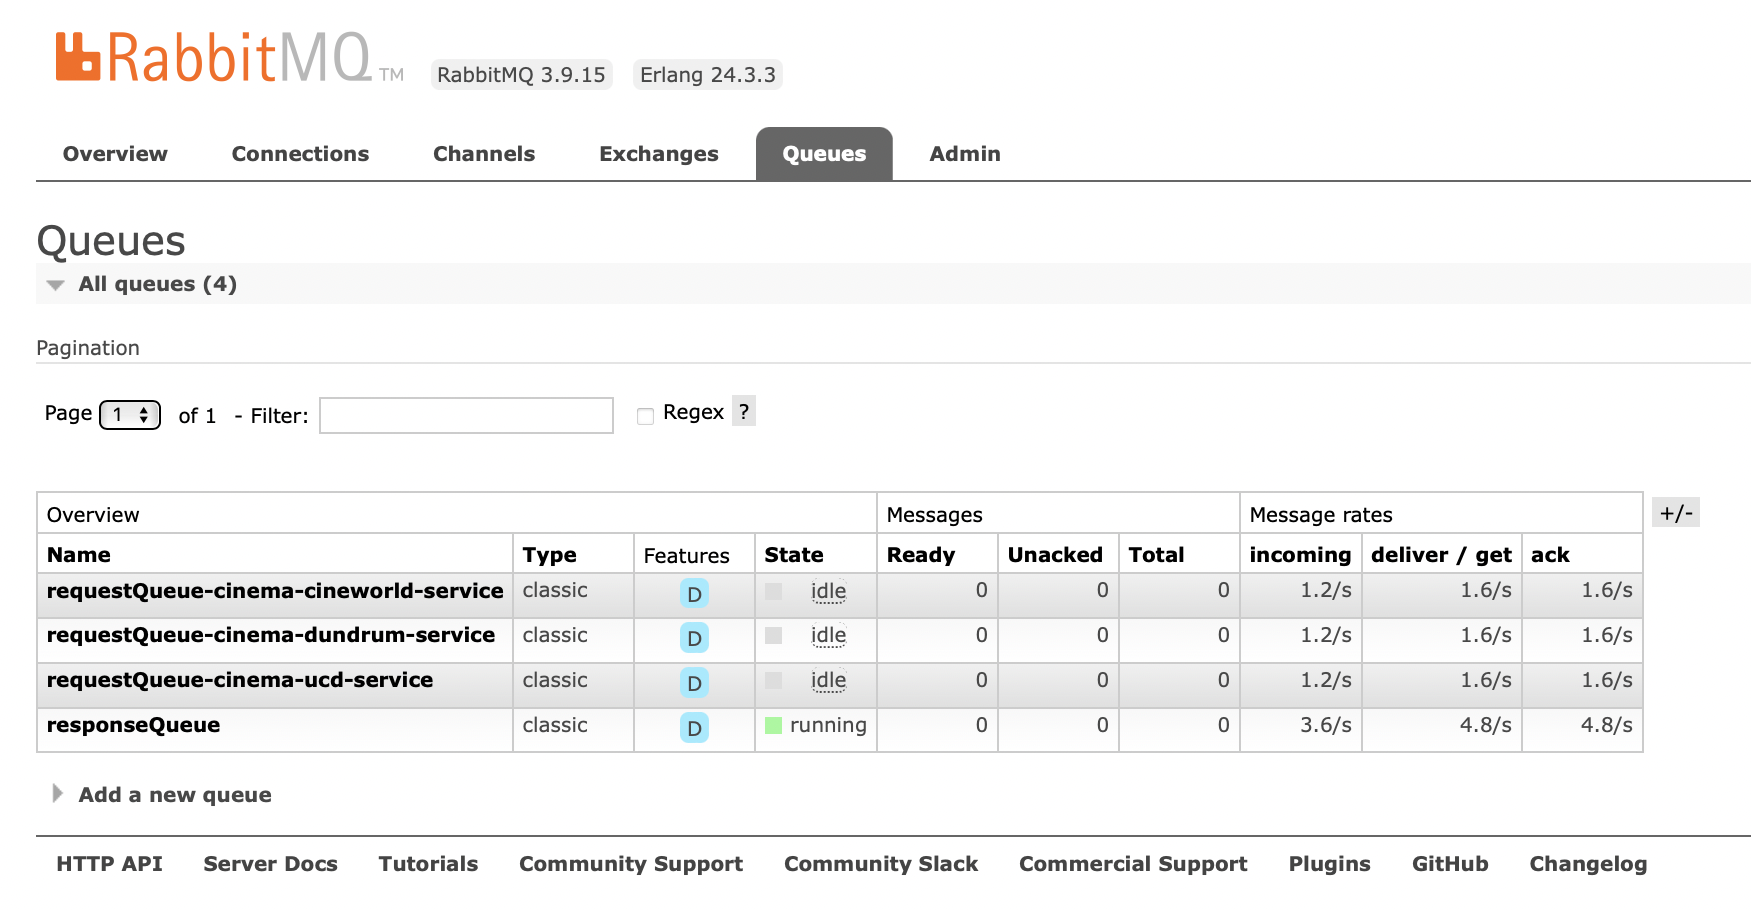
\includegraphics[width=1.0\linewidth]{./assets/images/case-studies/rmq-management.png}
  \caption{The Queues section from the RabbitMQ Management UI (\url{http://localhost:15672}). Default login credentials: \code{guest:guest}}
  \label{fig:rmq-management}
\end{figure}

In each microservice, a \code{config.MessagingConfig} \code{@Configuration} class defines the above infrastructure as Spring beans using Spring AMQP abstractions. As previously mentioned, the broker service exposes a synchronous REST API for the client. This is in fact a way to implement the asynchronous request/response pattern as seen in Fig. \ref{fig:async-req-res}). The first API call enqueues a request to be processed, and returns a temporary result like a new endpoint or the request ID that was forwarded. Then a second API call actually returns the data requested, after ensuring that the result is mapped to the correct request (usually using an ID).

\begin{figure}[H]
  \centering
  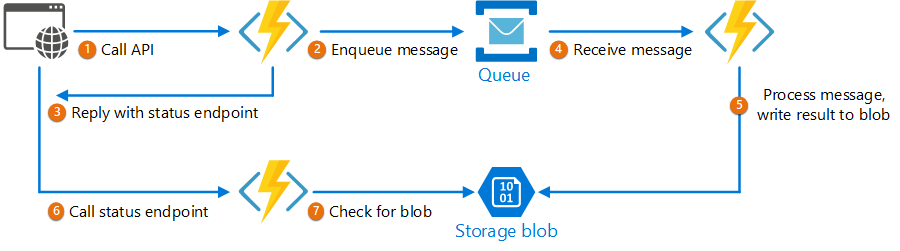
\includegraphics[width=0.8\linewidth]{./assets/images/case-studies/async-req-res.png}
  \caption{Sample asynchronous request/response pattern}
  \captionsource{Microsoft, \url{https://github.com/mspnp/cloud-design-patterns}}
  \label{fig:async-req-res}
\end{figure}

For example, one function of the system is to list the movie the showtimes from all cinemas. Instead of immediately returning the movies, the \code{/api/movie/list} endpoint simply broadcasts the request to all cinemas, and returns a broker-generated \textit{correlation ID}. This ID is used to map the asynchronous request to the responses. The broker uses a \code{@RabbitListener} to monitor the response queue, and any received messages are cached, ready to return to the client when the proper correlation ID is provided via the corresponding API endpoint: \code{/api/movie/list/\{correlationId\}}. Unlike the synchronous broker-client communication, the broker-cinema communication channels are completely asynchronous. A \code{RabbitTemplate} and \code{MessagePostProcessor} are used to format messages from the broker, and published to the appropriate queues for the cinemas. All plain Java objects are serialised by the message converter. The individual cinema services also use a \code{@RabbitListener} to monitor the request queue for broker requests, then perform database read/write operations, and finally route the response to the common response queue.

The code listing below shows a snippet from the broker service, with a HTTP GET mapping to send a request (e.g. listing movie showtimes from cinemas) and return a correlation ID \code{String}, then a separate GET mapping using the ID to fetch the response list asynchronously.


\begin{lstlisting}[language=Java, caption=Code snippet from \code{MovieController.java} in \code{broker-service}]
  @GetMapping("/list")
  public String listMovies() {
      String endpoint = "/movie/list";
      String routingKey = requestRoutingKey;
      String correlationId =
              brokerService.sendRequest(new RequestMessage(endpoint, null), routingKey);
      return correlationId;
  }

  @GetMapping("/list/{correlationId}")
  public List<Cinema> listMoviesResponse(@PathVariable String correlationId) {
      List<Message> responses = brokerService.fetchResponseFromCache(correlationId);
      return responses.stream()
              .map(r -> (Cinema) SerializationUtils.deserialize(r.getBody()))
              .collect(Collectors.toList());
  }
\end{lstlisting}

As mentioned earlier, any asynchronous responses from cinemas are first cached in the broker using the correlation ID, then the API allows reading from the cache with the correct ID via a separate endpoint. In terms of system performance compared to case study 1, there is no longer a need for the client to be blocked after sending a request (in anticipation of an immediate response). Requests can be sent to the broker, and then fetched later when needed using the correlation ID. As a result, the client can continue with other tasks after sending a series of requests to be processed, then collect the responses when they need to be displayed by some frontend.


\subsubsection{Application Metrics}

For successful performance engineering in a distributed system, observability and monitoring pattern implementations are indispensable. Monitoring is often defined as capturing the behaviour of a system by performing health checks and metrics over time, to aid the process of anomaly detection and root cause analysis. While maintaining text logs is also important, aggregated metrics over periods of time provide insights into the historical and current state of a system. In order to understand the behaviour of an application and be able to troubleshoot performance issues or service degradations, adequate monitoring infrastructure must be in place, along with visualisation tools.

In applications using RabbitMQ, the most popular monitoring stack includes Prometheus \footnote{\url{https://prometheus.io}} (monitoring toolkit) and Grafana \footnote{\url{https://grafana.com/grafana/}} (metrics visualisation). Although a default management plugin \footnote{\url{https://www.rabbitmq.com/management.html}} exists (exposing RabbitMQ metrics for nodes, connections, message rates, etc.), long term metric storage and visualisation services like Prometheus and Grafana are known to be more suitable for production systems.

The \code{rabbitmq\_prometheus} plugin exposes all RabbitMQ metrics on port 15692, in Prometheus text format. A dedicated Dockerised Prometheus server is also set up (configuration file: \code{prometheus.yml}) to monitor \textit{itself} (port 9090), the RabbitMQ prometheus metrics (port 15692) as well as a Dockerised \code{node-exporter} service (Prometheus exporter for host machine hardware and OS metrics) (port 9100). A screenshot of the Prometheus target dashboard is shown in Fig.
\ref{fig:prom-targets}, with the 3 targets defined in \code{prometheus.yml} for scraping metrics.

\begin{figure}[H]
  \centering
  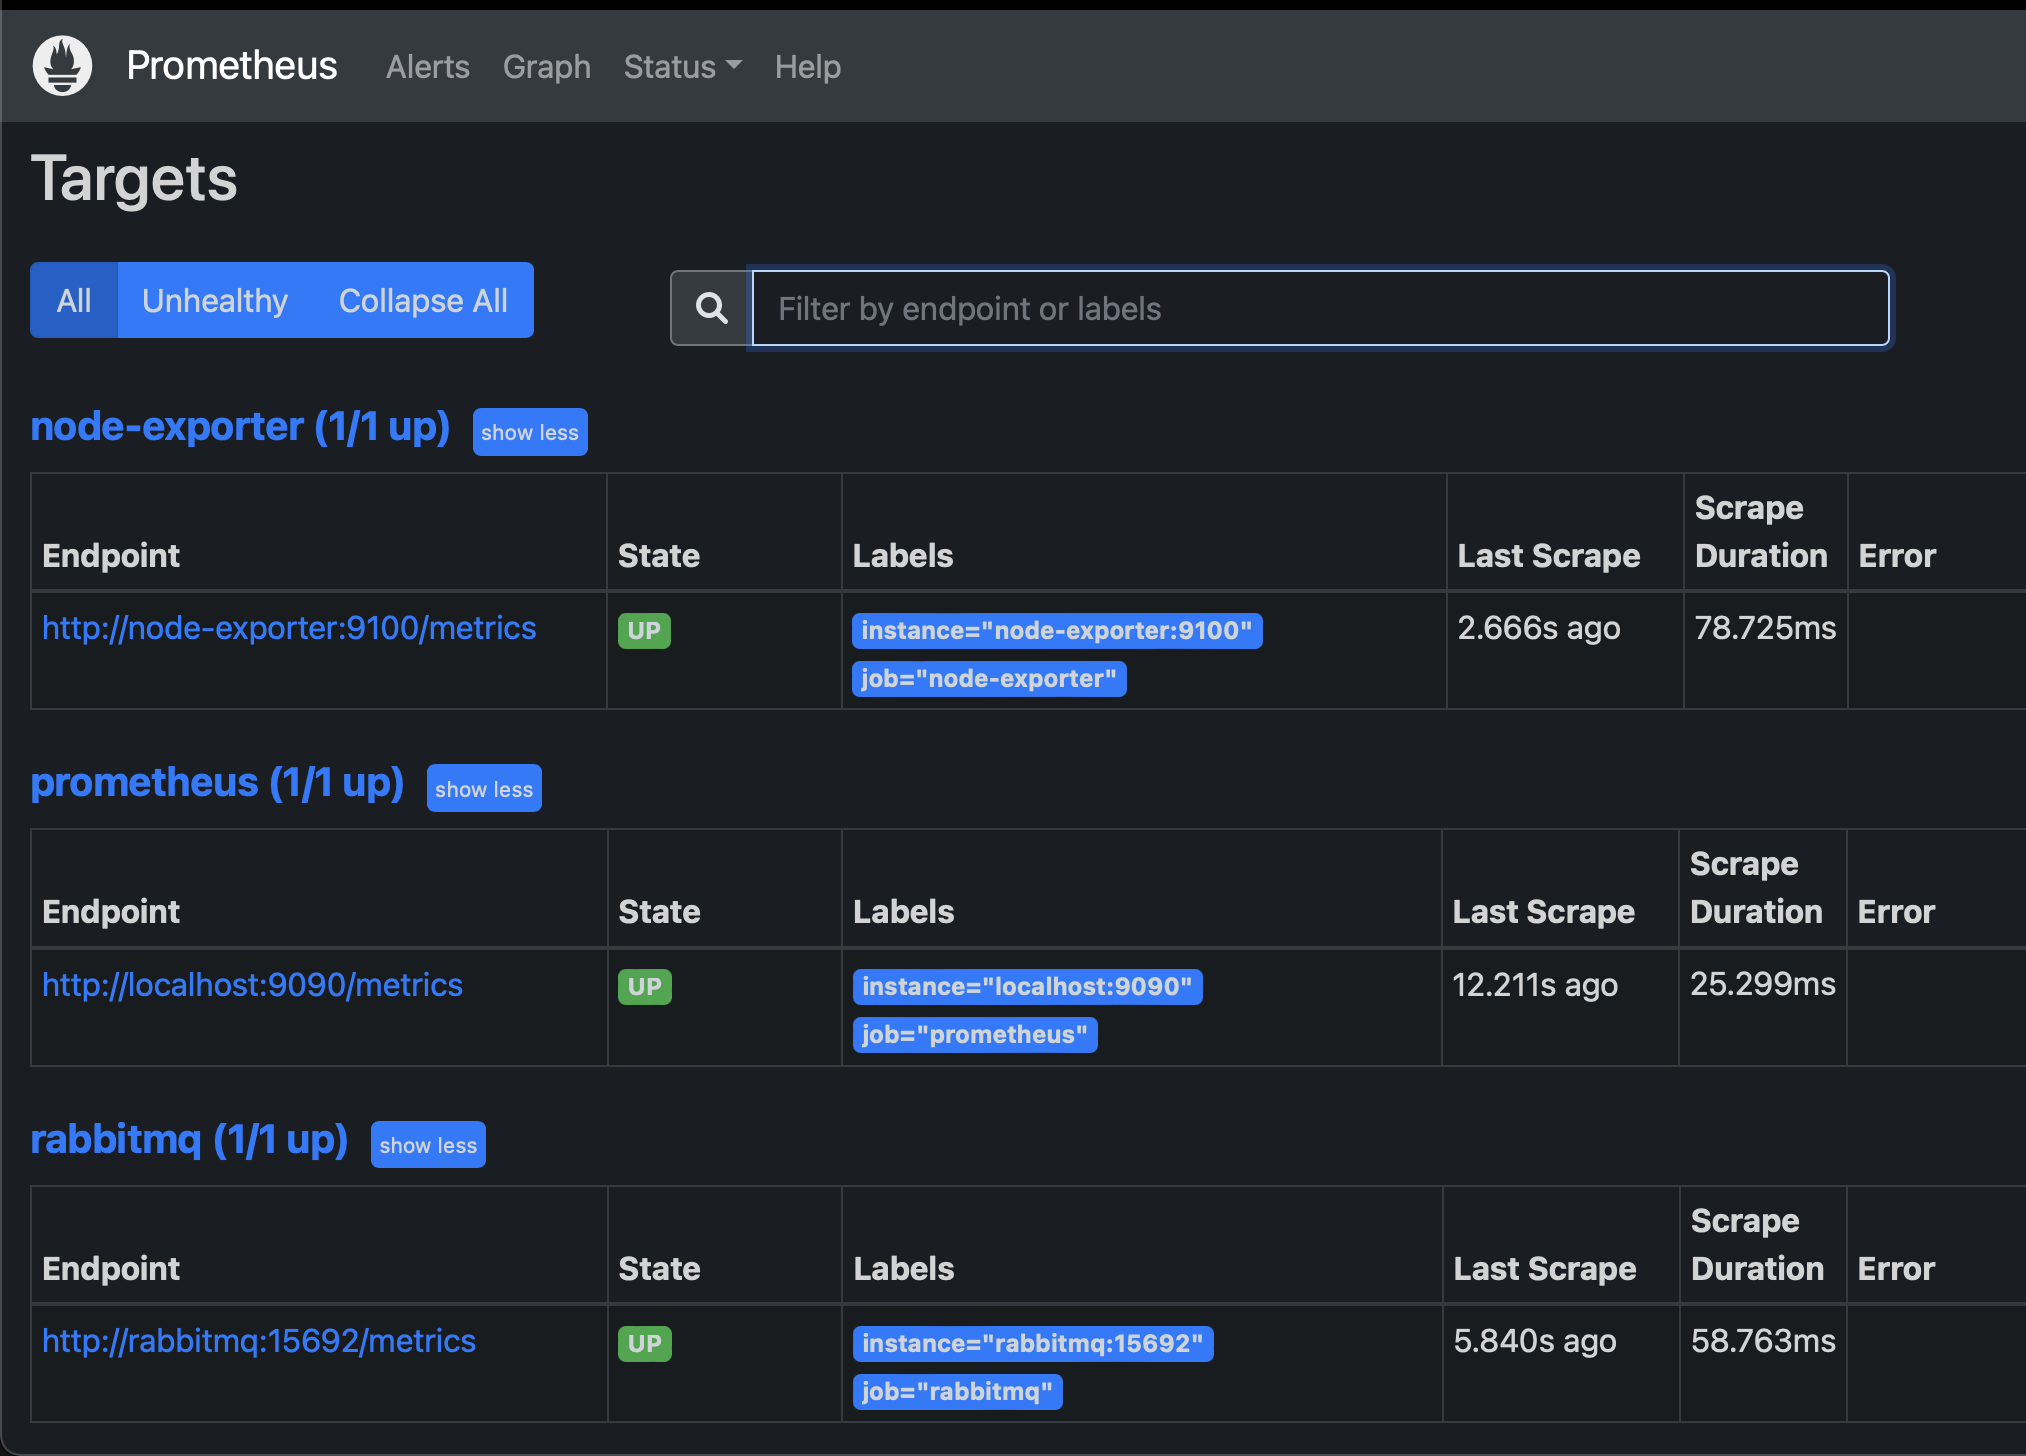
\includegraphics[width=0.75\linewidth]{./assets/images/case-studies/prom-targets.png}
  \caption{Prometheus targets dashboard on \url{http://localhost:9090}.}
  \label{fig:prom-targets}
\end{figure}

Due to the limited features of the RabbitMQ management plugin and the Prometheus dashboard alone, Grafana (port 3000, default credentials \code{admin:admin}) is the visualisation tool of choice, which can use the Prometheus server as a data source. The RabbitMQ team provides a number of pre-designed Grafana dashboards for RabbitMQ and runtime metrics (e.g. \code{RabbitMQ-Overview.json} shown in Fig. \ref{fig:grafana-overview}; runtime memory allocators, inter-node communication, etc.), which are specified in the local \code{./grafana/} directory.

\begin{figure}[H]
  \centering
  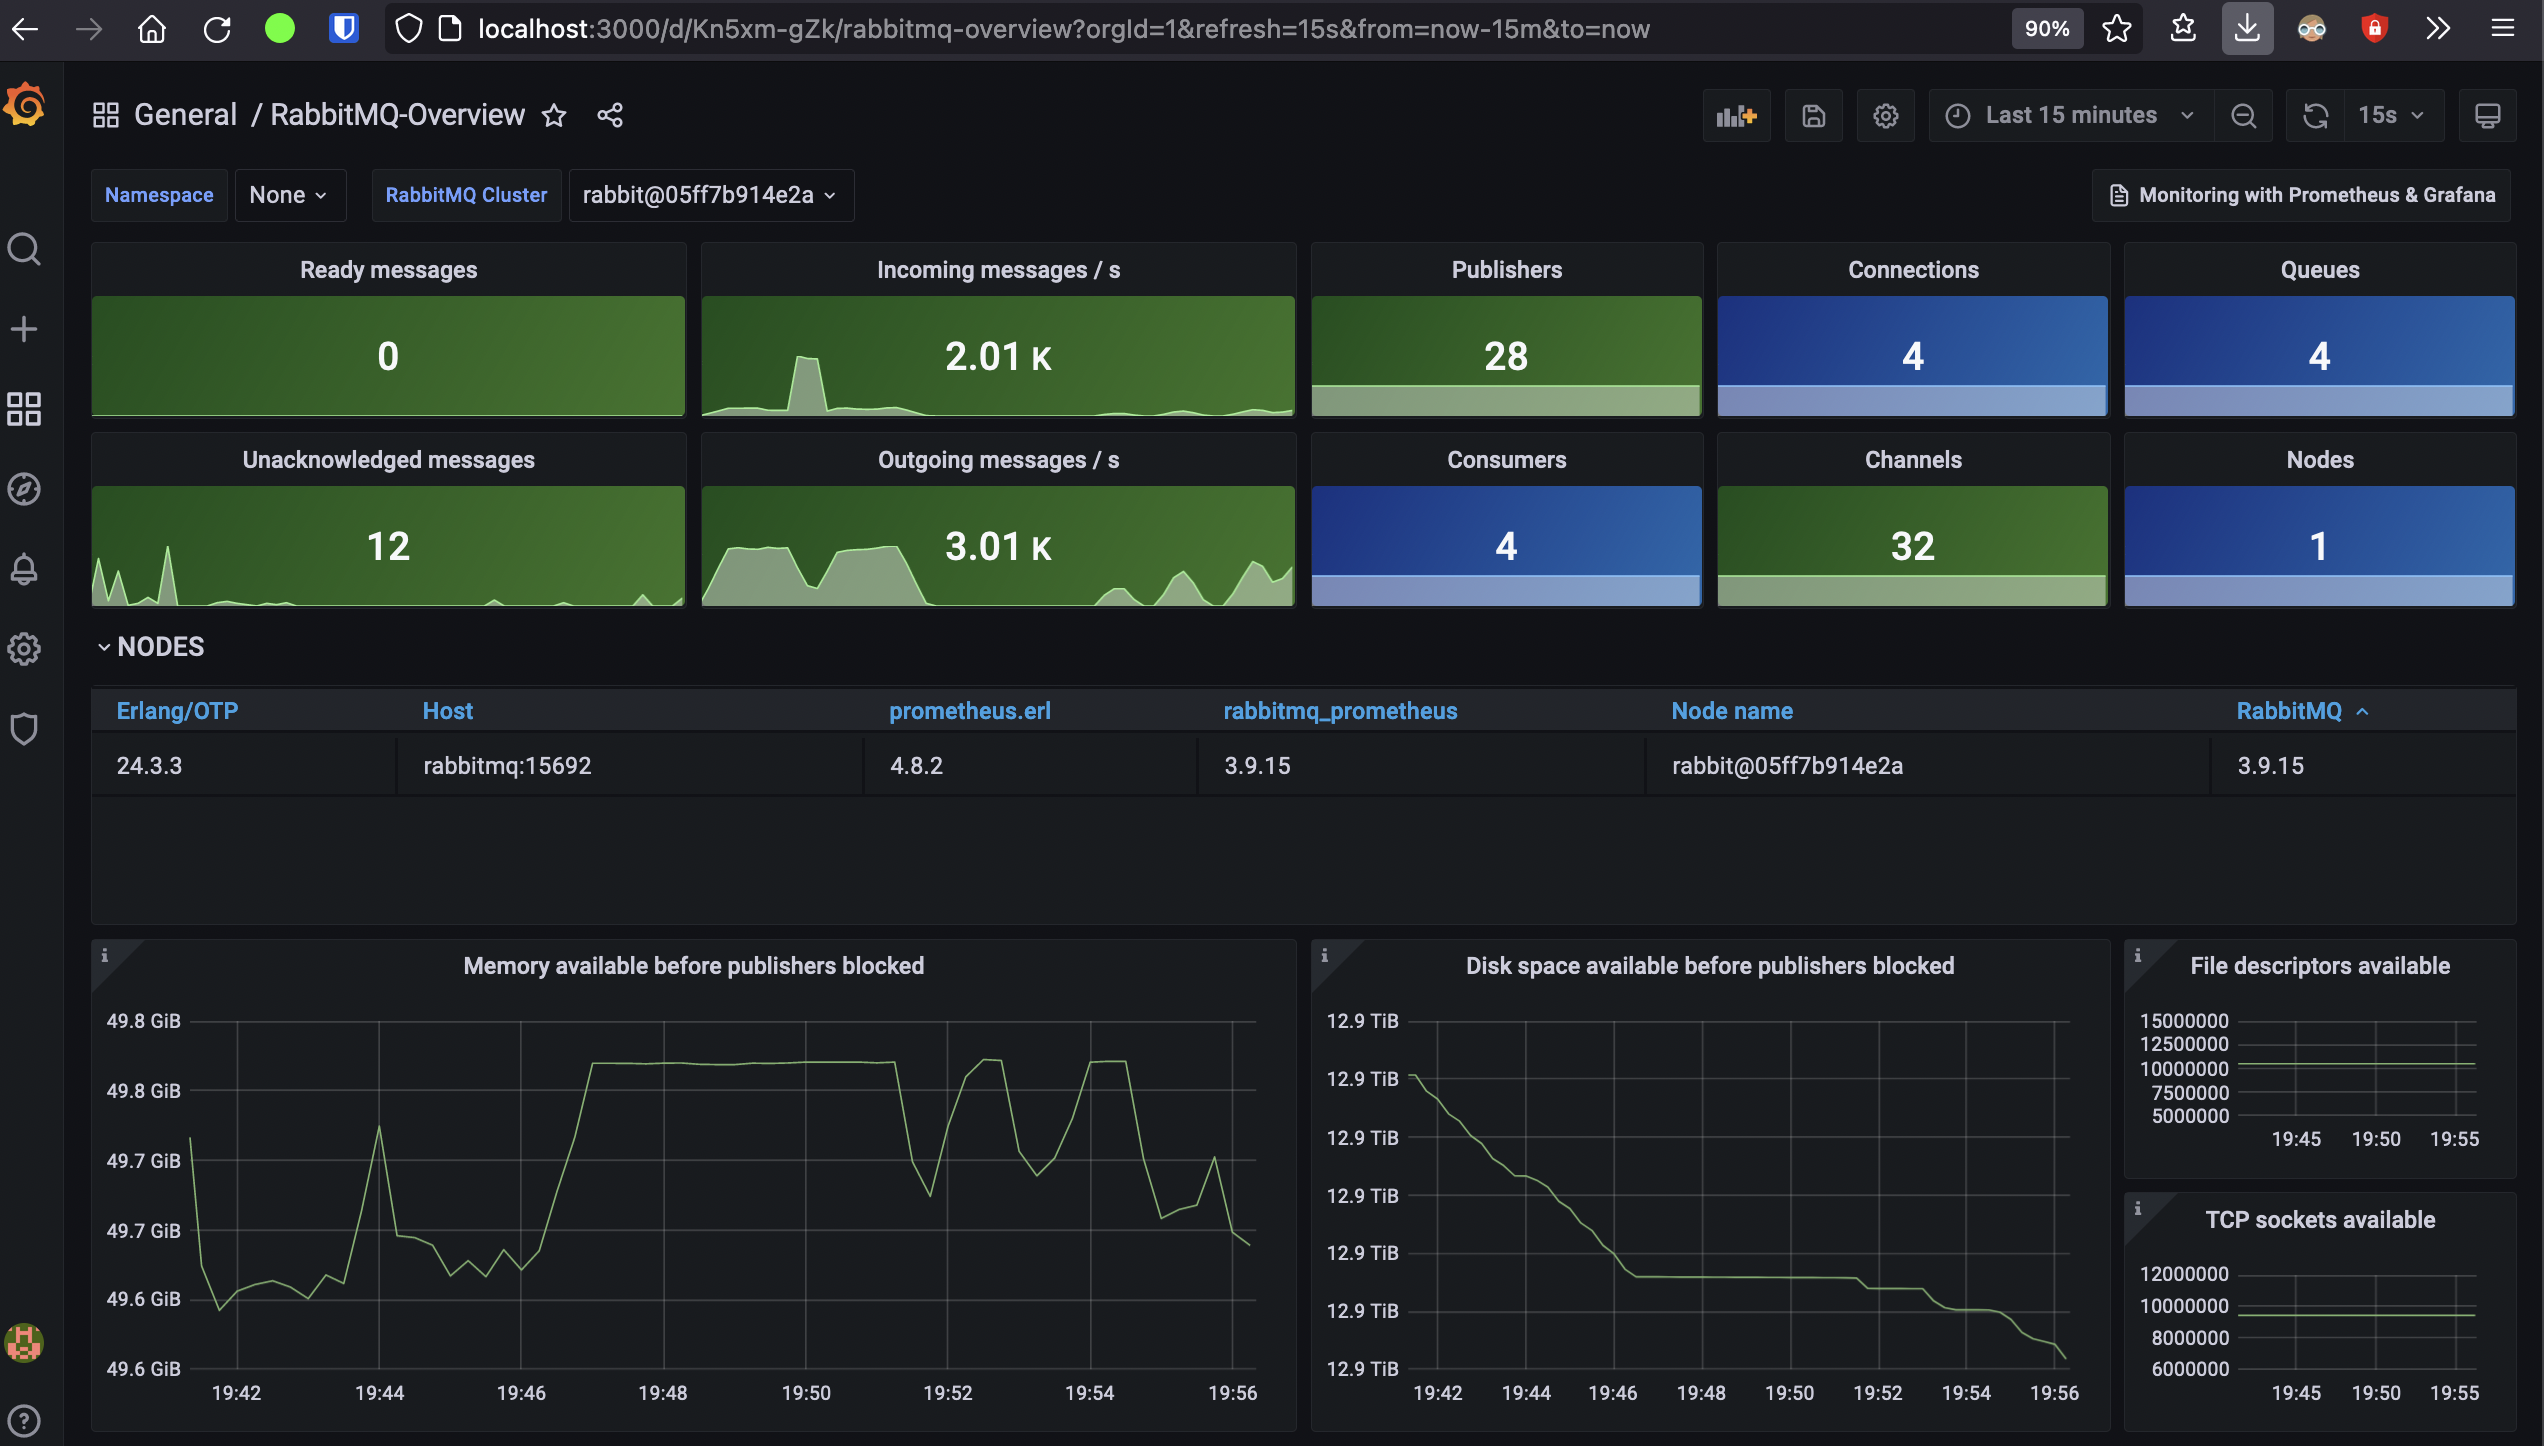
\includegraphics[width=1.0\linewidth]{./assets/images/case-studies/grafana-overview.png}
  \caption{Grafana RabbitMQ overview dashboard on \url{http://localhost:3000} during a load test.}
  \label{fig:grafana-overview}
\end{figure}


\subsubsection{Health Check API}

As discussed earlier, monitoring is crucial for any application, the basic aspect of which happens to be \textit{health checking}. This is especially true for modern-day microservices, which are usually hosted on the cloud: affected by several factors such as network latency, bandwidth, and performance of "black-box" host machines. Hence, the health of services should be verified regularly as a part of the monitoring infrastructure, in order to maintain SLAs (service level agreement) and necessary availability levels.

The RabbitMQ HTTP API reference, including details on health check endpoints, is available here \footnote{\url{https://pulse.mozilla.org/api/index.html}}. The functioning of the following health check endpoints (with status code 200 if healthy) is demonstrated (using VS Code's REST Client) in supplementary figures:

\begin{itemize}
  \item \code{/api/health/checks/alarms} (Fig. \ref{fig:cs02-hc1}): Responds a 200 OK if there are no alarms in effect in the cluster, otherwise responds with a 503 Service Unavailable.
  \item \code{/api/health/checks/certificate-expiration/\{within\}/\{unit\}} (Fig. \ref{fig:cs02-hc3}):  Checks the expiration date on the certificates for every listener configured to use TLS. Responds a 200 OK if all certificates are valid (have not expired), otherwise responds with a 503 Service Unavailable. Valid units: days, weeks, months, years. The value of the within argument is the number of units. So, when within is 2 and unit is "months", the expiration period used by the check will be the next two months.
  \item \code{/api/health/checks/protocol-listener/\{protocol\}} (Fig. \ref{fig:cs02-hc5}): Responds a 200 OK if there is an active listener for the given protocol, otherwise responds with a 503 Service Unavailable. Valid protocol names are: amqp091, amqp10, mqtt, stomp, web-mqtt, web-stomp.
\end{itemize}

A few other useful endpoints are listed here, with details available in the API reference:
\begin{itemize}
  \item \code{/api/health/checks/local-alarms}
  \item \code{/api/health/checks/port-listener/\{port\}}
  \item \code{/api/health/checks/virtual-hosts}
  \item \code{/api/health/checks/node-is-mirror-sync-critical}
  \item \code{/api/health/checks/node-is-quorum-critical}
\end{itemize}


The next three design patterns are invaluable to a microservice-based application like the one implemented in case studies 1 and 2, and are hence common to both:

\subsubsection{Externalised Configuration}

Docker Compose environment variables and Spring application properties for the various services are used to configure the microservices. The environment variables set by Docker are translated into Spring Boot application properties, e.g. \code{SERVER\_PORT} becomes \code{server.port}, \code{SPRING\_RABBITMQ\_HOST} becomes \code{spring.rabbitmq.host}, etc. without even having to specify the properties in the standard \code{application.yml}.

\begin{lstlisting}[caption=UCD cinema's \code{application.yml}]
  spring:
    application:
      name: cinema-ucd-service

  data_file: data/movies.json

  amqp:
    exchange: cinema
    request:
      routingKey: request.to.cinema
      serviceOnlyRoutingKey: request.to.cinema.ucd
    response:
      routingKey: response.from.cinema
\end{lstlisting}

The listing above shows how the data file used to populate MongoDB, and other RabbitMQ configurations such as name of exchange and routing keys are set in the application properties. When access is required in the source code, Spring uses the \code{@Value} annotation to read said properties. As mentioned in case study 1, externalising configuration in this manner helps with organisation and reduces avoidable development (human) errors.

\subsubsection{Database per Service}

Maintaining a separate MongoDB database for each cinema microservice is still the most practical approach in a distributed system to avoid a data operation bottleneck. A server is set up with Docker, and multiple databases are created again with the help of Spring Boot environment variables such as \code{SPRING\_DATA\_MONGODB\_DATABASE} and \code{SPRING\_DATA\_MONGODB\_PORT}.

\begin{lstlisting}[caption=Snippet from \code{docker-compose.yml} for UCD cinema]
  cinema-ucd-service:
    ...
    environment:
      ...
      - SPRING_DATA_MONGODB_HOST=mongodb
      - SPRING_DATA_MONGODB_DATABASE=cinema-ucd
      - SPRING_DATA_MONGODB_PORT=27017
    ...
\end{lstlisting}

\subsubsection{Service Instance per Container}

The ease of spinning up Docker containers makes this deployment pattern the industry standard for microservices. This is especially true for this second case study, where much additional infrastructure is required, such as RabbitMQ messaging system, Prometheus and Grafana servers for monitoring, which are all deployed as independent Dockerised services. Exposing ports such as 9090 (Prometheus), 3000 (Grafana), 15672 (RabbitMQ management) provides access to various user interfaces to host machine browsers. Using Docker Swarm or Kubernetes with Docker allows container scaling and orchestration, which are important when the load creates a need for multiple containers across multiple host machines.

\subsection{Evaluation}

Similar to the previous case study, the same approach of modelling, manual API testing and JMeter load testing is adopted here.

\subsubsection{Performance Modelling}

The significant change in communication mechanism from synchronous REST alone (case study 1), to asynchronous request/response (external) and messaging (internal) is expected to yield performance benefits. Fig. \ref{fig:cs02-sequence} shows quite a different sequence diagram for the identical movie listing use case explored in case study 1's evaluation.

\begin{figure}[H]
  \centering
  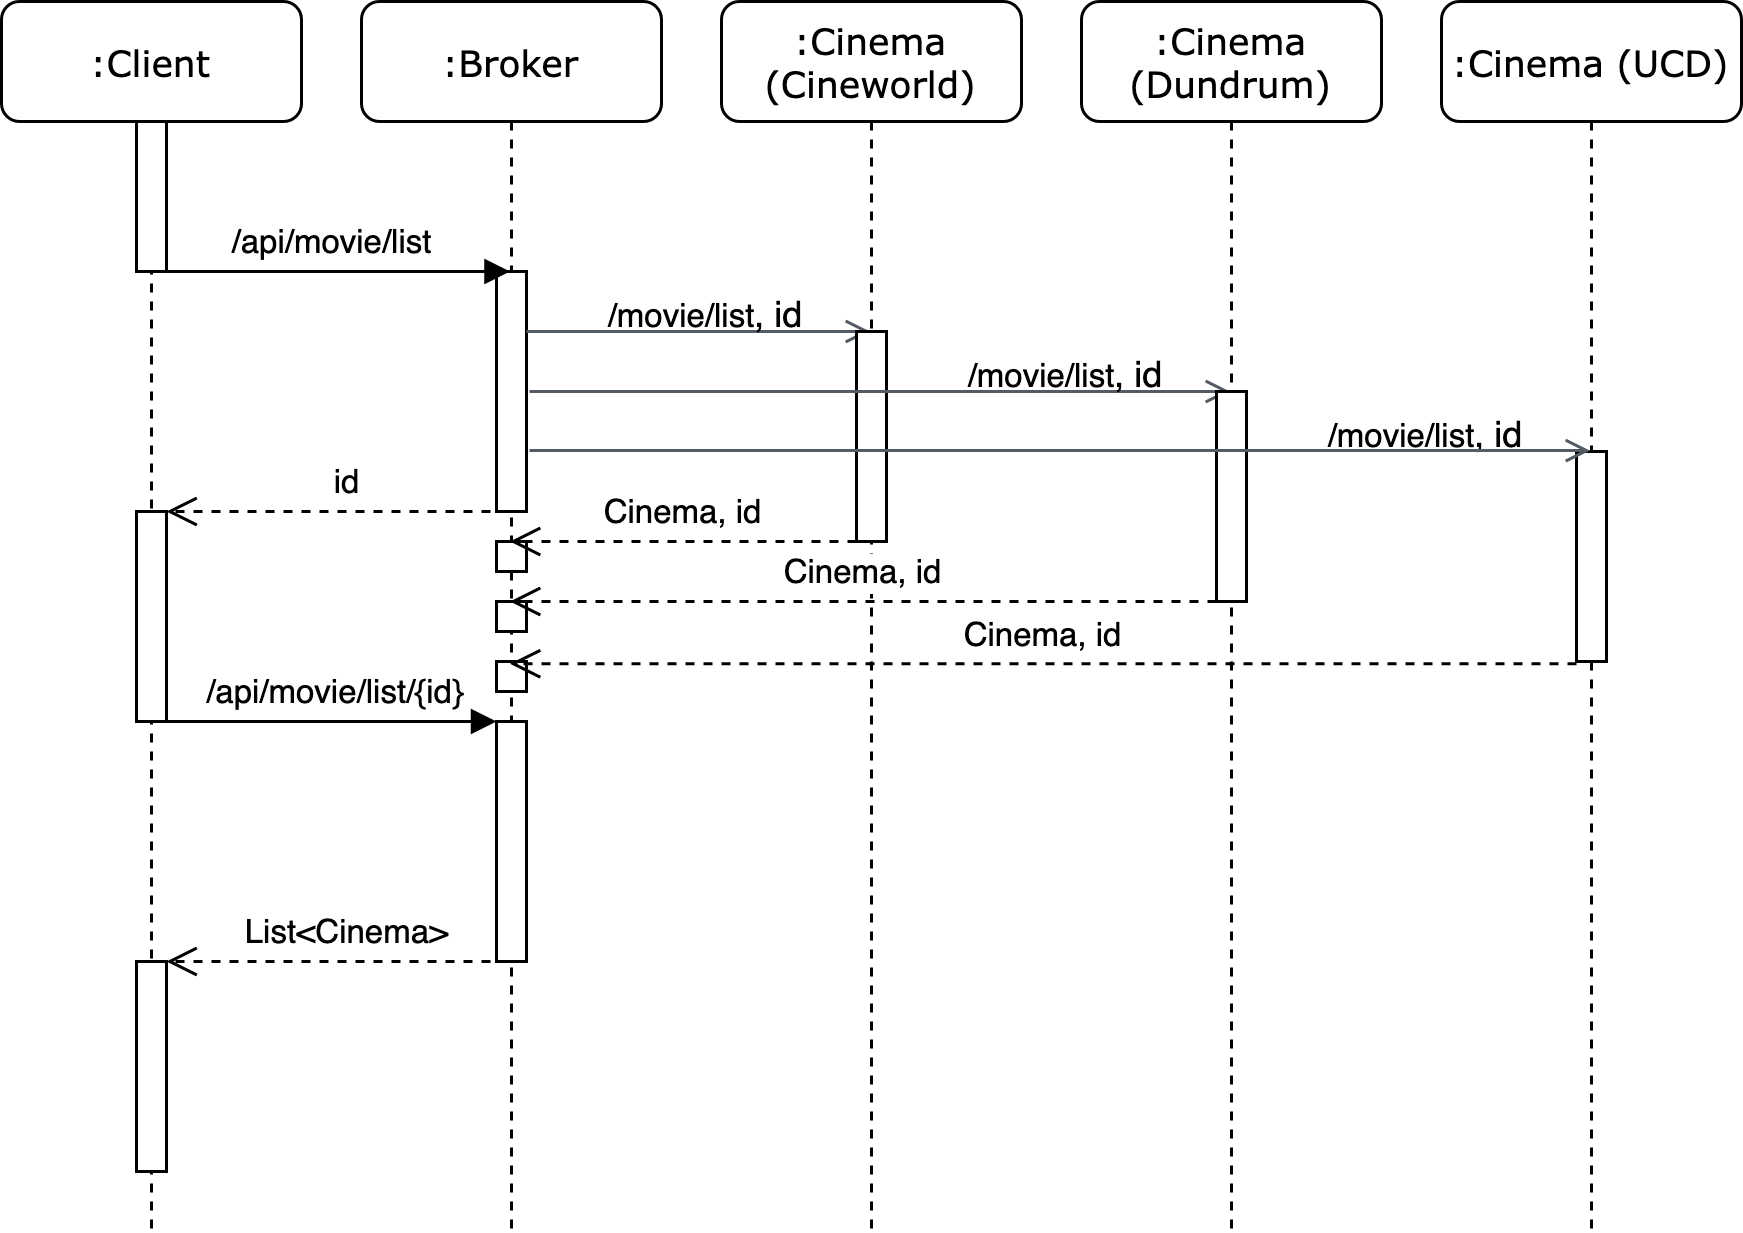
\includegraphics[width=0.75\linewidth]{./assets/diagrams/cs02-sequence.png}
  \caption{UML sequence diagram for listing movies from all cinemas (case study 2).}
  \label{fig:cs02-sequence}
\end{figure}

Sequence of steps:
\begin{itemize}
  \item Firstly, contacting the Broker via synchronous REST only returns a correlation ID of the forwarded request, instead of a list of movies.
  \item Next, the Broker sends asynchronous messages (open arrow heads, solid lines) to each Cinema via the RabbitMQ infrastructure (topic exchange, queues, routing keys), without expecting an immediate response.
  \item When a Cinema is done processing the request, it returns the list of movie showtimes to the Broker, along with the request ID.
  \item The Broker caches the responses from Cinemas using the same correlation ID, ready to be requested by the Client.
  \item When the Client makes another synchronous REST API call to the Broker with the appropriate ID, the Broker returns any responses that were cached in the time since the initial request.
\end{itemize}

The above model suggests the possibility of higher overall system performance compared to the first case study, since all inter-service communication is asynchronous and non-blocking. This is in fact a well-accepted approach when dealing with microservice-architecture - to have the external client or frontend facing service (like the broker) expose a synchronous REST API, while the internal microservices (like the cinemas with the broker) communicate asynchronously (here, via message queues).
Requests are linked to their corresponding responses by some form of correlation ID. However, care must still be taken to scale the Broker service as needed to handle increasing load, since it is the single point of entry for external clients.

\subsubsection{Manual API Testing}

Again, using VS Code's REST Client, various HTTP requests (stored under \code{src/main/resources/http/}) to the client-facing Broker service (port 8099) are timed. Internal cinema services use RabbitMQ queues, a topic exchange and routing keys to pass messages to/from the central Broker. The following endpoints have been tested to demonstrate the functionality of the web application:

\begin{itemize}
  \item \code{/api/movie/list} (Fig. \ref{fig:cs02-manual-1}): The \code{/list} endpoint sends a request to the Broker to list the movie showtimes from all cinema services. Since the Broker communicates with the cinemas via asynchronous messaging, only an alphanumeric series of characters (separated by hyphens) is returned by the GET request (in 160 ms), which is the request's correlation ID.

  \item \code{/api/movie/list/\{correlationId\}} (Fig. \ref{fig:cs02-manual-2}): On providing the same correlation ID received earlier as a path variable in a new GET request, the full list of movie showtimes from all cinemas is returned (in 78 ms). The Broker uses the time between the two requests to cache responses from any cinemas that are able to process the request in the given time-frame.

  \item \code{/api/cinema/cineworld/reservation/make} (Fig. \ref{fig:cs02-manual-3}): A targeted request to the Cineworld cinema must also go via the message Broker (\code{/api} prefix), unlike the first case study where such as request is directly sent to the appropriate cinema via an API gateway. Here, the Broker creates a custom routing key to forward the request only to the appropriate cinema's request queue, instead of broadcasting it to all queues. A POST request to Cineworld contains booking details identical to those seen in the first case study, and a correlation ID is returned in 65 ms.

  \item \code{/api/cinema/cineworld/reservation/make/\{correlationId\}} (Fig. \ref{fig:cs02-manual-4}): A GET request to the \code{/reservation/make} endpoint with the appropriate correlation ID yields a response in 31 ms with the successful reservation details.

  \item \code{/api/cinema/cineworld/reservation/list} (Fig. \ref{fig:cs02-manual-5}): It only takes 10 ms to fetch the correlation ID for a reservation list GET request to Cineworld.

  \item \code{/api/cinema/cineworld/reservation/list/\{correlationId\}} (Fig. \ref{fig:cs02-manual-6}): In 13 ms, the server is able to list all the reservations at Cineworld, thus confirming the success of the earlier \code{/reservation/make} request.
\end{itemize}

This asynchronous request/response pattern is especially useful in preventing client blocking (as seen in the first case study), since the client is now able to perform other tasks after sending a series of requests to the Broker, without having to wait for every single request to receive a full response before moving on.


\subsubsection{Performance Testing}

Using JMeter again, two load tests (A and B) were designed in a similar fashion to case study 1. However, due to the asynchronous nature of communication in case study 2, each test plan includes two HTTP requests: one to send the initial request to the Broker and get a correlation ID, and another to use the correlation ID to fetch the final response. A regular expression extractor (post-processor) is used in JMeter to extract the correlation ID from the response body after the first request, then use it as a path variable for the second request. Other test parameters are identical to case study 1, for instance: constant load increments from 10 to 100 threads, 1 seconds ramp-up, and 1000 test iterations at each load level for reliability.

\begin{figure}[H]
  \centering
  \subfigure[]{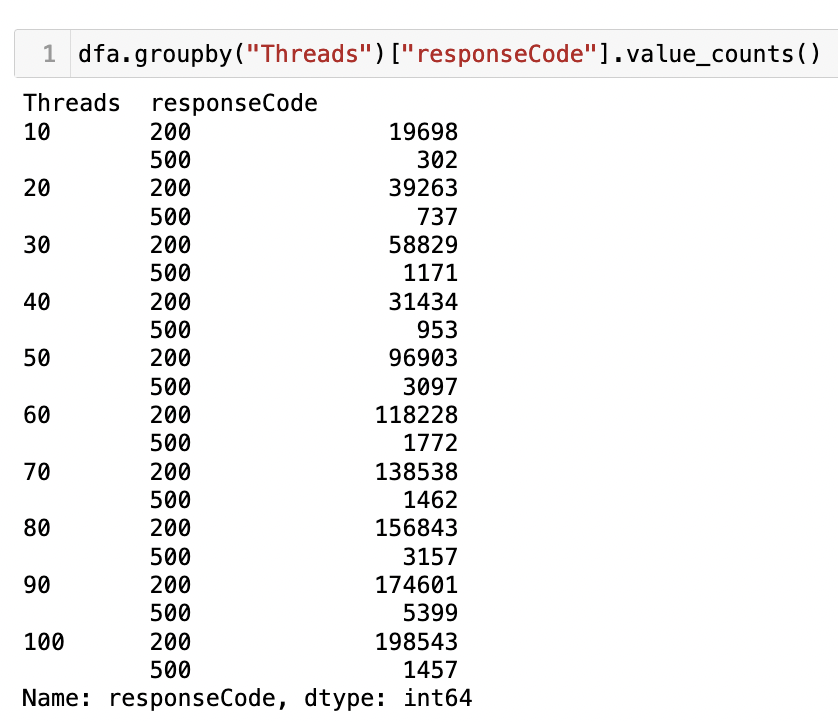
\includegraphics[width=0.45\linewidth]{./assets/images/case-studies/cs02-lta-1.png}}
  \subfigure[]{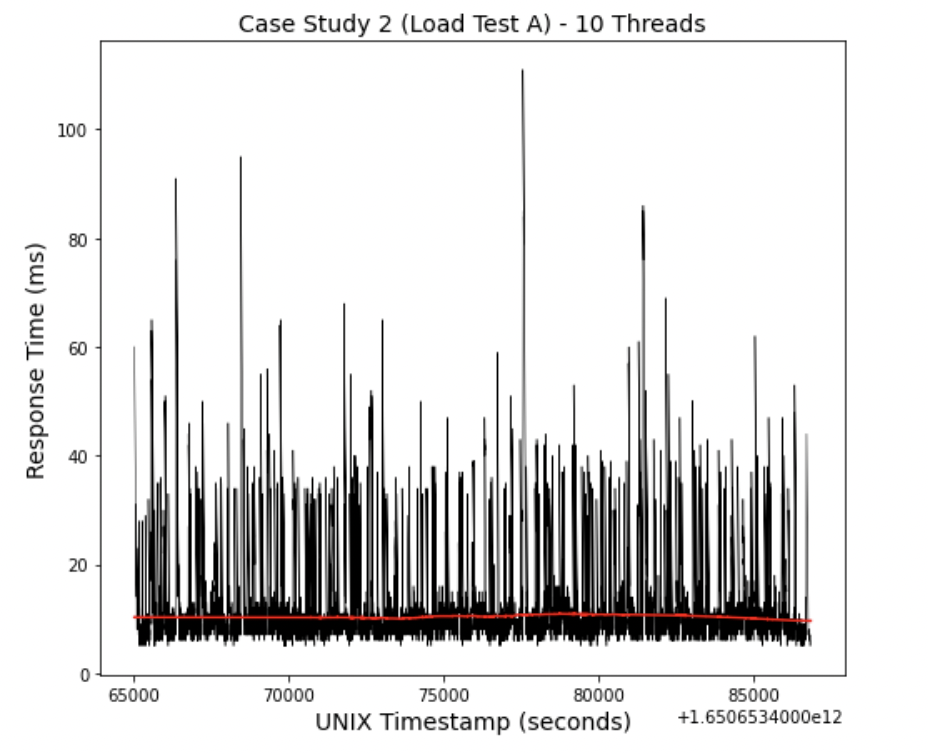
\includegraphics[width=0.45\linewidth]{./assets/images/case-studies/cs02-lta-2.png}}
  \caption{Load test A response times using (a) 10 threads and (b) 100 threads.}
  \label{fig:cs02-lta-12}
\end{figure}

Load test A involves the Broker API endpoints \code{/api/movie/list} and \code{/api/movie/list/\{correlationId\}}. As seen in Fig. \ref{fig:cs02-lta-12}, the response time at both load levels - 10 threads and 100 threads - are far more variable, but lower on average compared to the case study 1 observations, but applying a Savitzky-Golay filter (red line) as before helps smoothen the data points for more readable plots. Both load scenarios show constant response times approximately under 10 ms and 75 ms - both lower than the case study 1 observations for identical loads. Tuning the RabbitMQ queue configurations (e.g. resource allocations) to better suit the system under test would reduce the variability in response times.

Fig. \ref{fig:cs02-lta-3} shows far lower error probabilities in case study 2 load test A requests, compared to those in case study 1. The absolute total response numbers are double that of case study 1 since there are two requests involved in each step - receiving the correlation ID, then using it in a subsequent request. A naive assumption incorporated into the test plan is that the Broker is able to finish caching the response before the second request to get the full response is received - and this is shown to be true for the vast majority of cases (the few failures are depicted by the 500 server error code numbers in the table). However, a better approach would be to separate the consecutive requests with a fixed wait period, and disregard the wait time when plotting average response times and calculating other metrics. The idea behind asynchronous requests as shown here is that the client does not require an immediate response to a query, but emulating such a scenario is difficult when response timing is involved while invoking a synchronous REST API and keeping track of correct correlation IDs.

\begin{figure}[H]
  \centering
  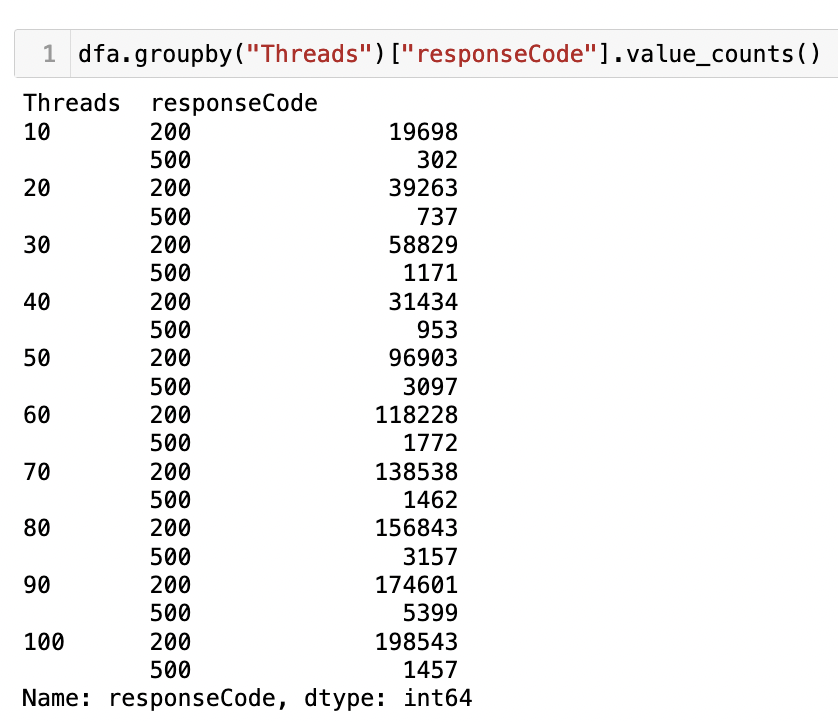
\includegraphics[width=0.5\linewidth]{./assets/images/case-studies/cs02-lta-3.png}
  \caption{Count of HTTP response codes during load test A at different load levels.}
  \label{fig:cs02-lta-3}
\end{figure}

Finally, a familiar linear plot with high Pearson correlation of 0.998 in Fig. \ref{fig:cs02-lta-4} confirms the linearity of resource utilisation with respect to load. An exponential curve instead would be indicative of a struggling system under constant load increments.

\begin{figure}[H]
  \centering
  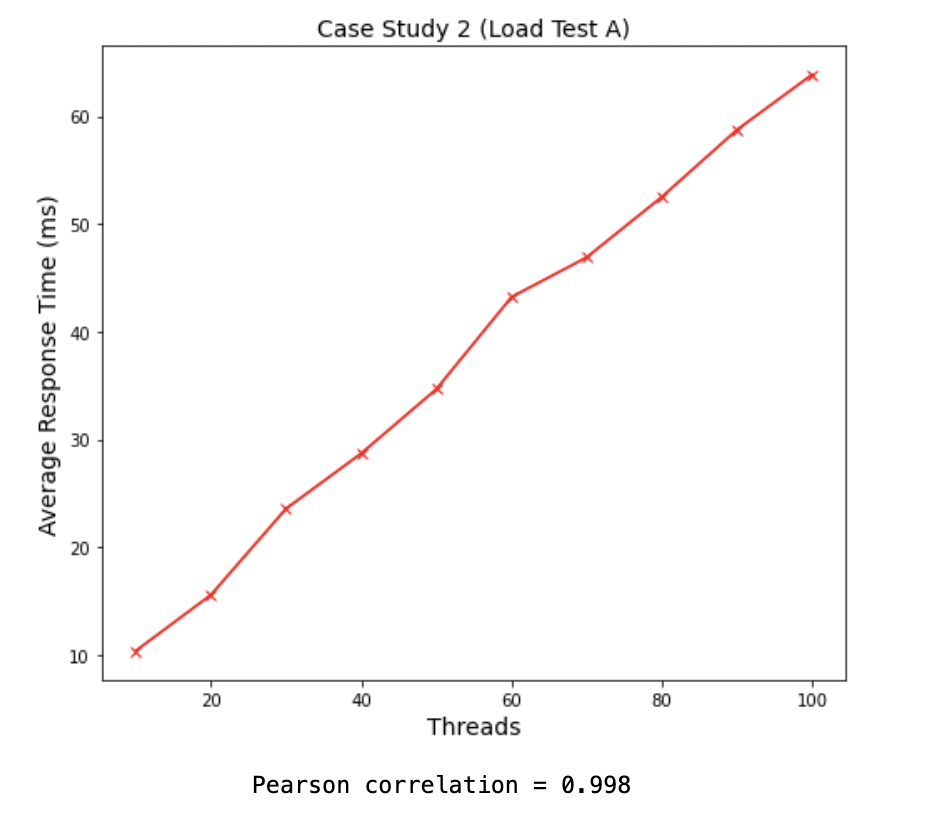
\includegraphics[width=0.55\linewidth]{./assets/images/case-studies/cs02-lta-4.png}
  \caption{Average response time vs number of threads in load test A.}
  \label{fig:cs02-lta-4}
\end{figure}

Load test B is designed to check the ticket reservation functionality, corresponding to endpoints \code{/api/cinema/cineworld/reservation/make} and \code{/api/cinema/cineworld/reservation/make/\{correlationId\}}, with an identical client booking payload (Jane Doe, Cineworld) for POST requests. The seconds request in each step is simple GET request with the extracted correlation ID as a path variable.

\begin{figure}[H]
  \centering
  \subfigure[]{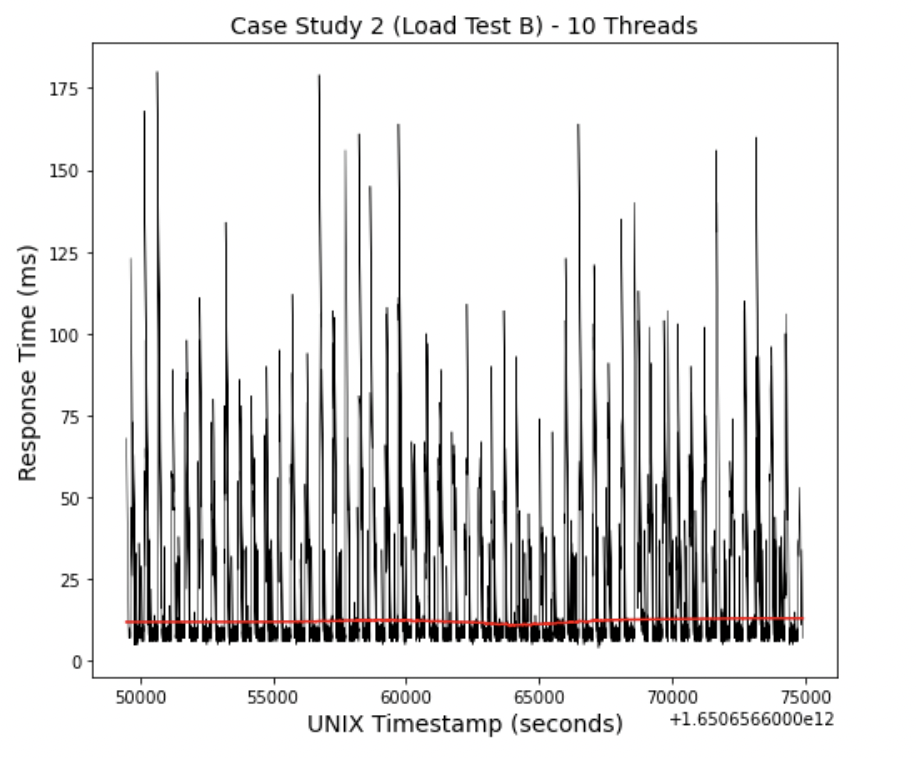
\includegraphics[width=0.4\linewidth]{./assets/images/case-studies/cs02-ltb-1.png}}
  \subfigure[]{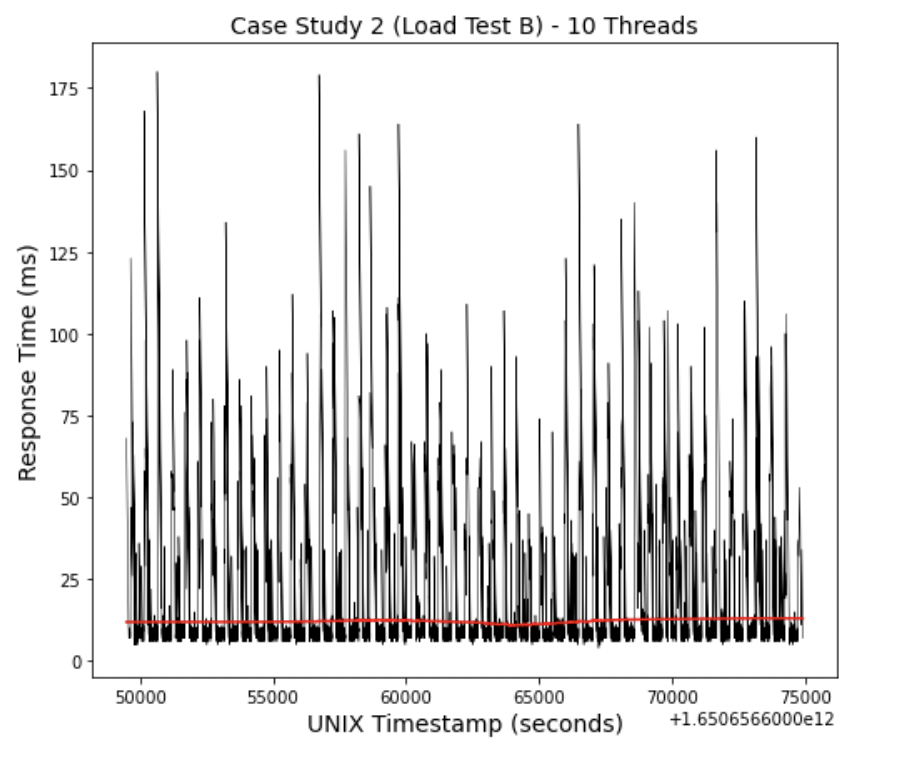
\includegraphics[width=0.45\linewidth]{./assets/images/case-studies/cs02-ltb-2.png}}
  \caption{Load test B response times using (a) 10 threads and (b) 100 threads.}
  \label{fig:cs02-ltb-12}
\end{figure}

Fig. \ref{fig:cs02-ltb-12} shows highly variable response times, but mostly constant Savitzky-Golay smooth red curves, measured at approximately 10 ms and 50 ms for load levels of 10 threads and 100 threads respectively. In this case, the average response times were higher that those in the previous case study, possibly due to the effect of two communication round trips, and request/response travel via a congested Broker service. This suggests that the Broker and RabbitMQ queues need to be configured with greater hardware resources to avoid a performance bottleneck.

Since the POST and GET requests were performed without a time gap in between, there is a small percentage of errors observed here, while there were none in case study 1. As mentioned earlier, these errors are caused in cases where the Broker doesn't finish storing microservice responses for some correlation IDs, and consequently the client cannot access the endpoint by providing an ID. Scaling the services is a plausible solution, since the prerequisite is satisfied - resource utilisation levels are directly proportional to the system load (Pearson correlation of 0.992 between average response time and number of threads in the load test).

\begin{figure}[H]
  \centering
  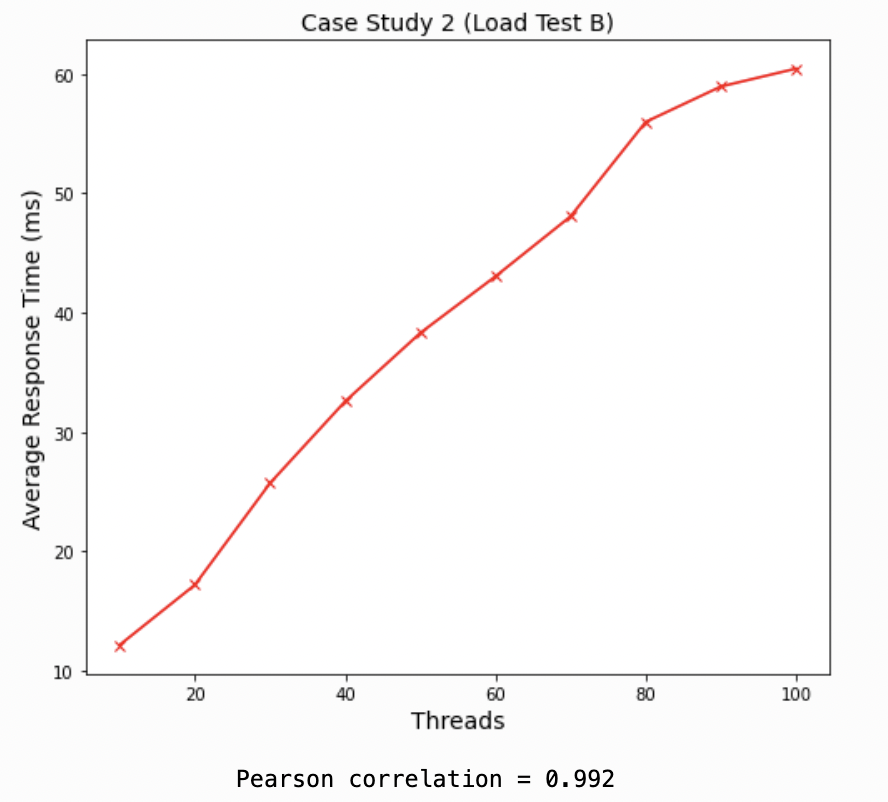
\includegraphics[width=0.55\linewidth]{./assets/images/case-studies/cs02-ltb-4.png}
  \caption{Average response time vs number of threads in load test B.}
  \label{fig:cs02-ltb-4}
\end{figure}
